\documentclass[a4paper, 12pt]{article}

\usepackage{cmap}
\usepackage[T2A]{fontenc}
\usepackage[utf8]{inputenc}

\usepackage{amsmath, amsfonts, amssymb, amsthm, mathtools}
\usepackage{icomma}

\title{Отчет о выполнении лабораторной работы \\ Эксперементадльная проверка закона вращательного движения на крестообразном маятнике}
\author{Лепарский Роман}
\date{08.11.2020}

\begin{document}

\maketitle

\newpage

\section{Аннотация}

Целью работы является получение зависимости углового ускорения от момента прикладываемых к маятнику сил. Необходимо убедиться, что угловое ускорение зависит от момента сил линейно, определить момент инерции маятника. Также, нужно проанализировать влияние сил трения, действующих на ось вращения.

\section{Теоретические сведения}

В данной работе эксперементально поверяется уравнение вращательного движения:
\begin{equation} \label{eq:main}
I\frac{d\omega}{dt} = M
\end{equation}

Для этого используется крестообразный маятник

\begin{center}
\includegraphics[scale = 0.3]{"pendulum.eps"}
\end{center}

Массы грузов:
\begin{center}
\begin{tabular}{|l|l|}
\hline
$m_1$, г & 155,5 \\ \hline
$m_2$, г & 148,9 \\ \hline
$m_3$, г & 151,9 \\ \hline
$m_4$, г & 150,1 \\ \hline
\end{tabular}
\end{center}

\[
m_0 = <m> = \frac{1}{N}\sum_{i=1}^N m_i = \frac{155,5+148,9+151,9+150,1}{4} = 151,6\text{г} 
\]

Запишем также некоторые полезные данные:
\begin{itemize}
	\item Высота опускания груза $H = 60$см
	\item Радиус маленького шкива $r_1 = 9$мм
	\item Радиус большого шкива $r_2 = 17,5$мм
	\item Расстояние от оси вращения до центров масс грузов в 1 опыте $R_1 = 60 + 12,5 = 72,5$мм
	\item Расстояние от оси вращения до центров масс грузов во 2 опыте $R_1 = 200 + 12,5 = 212,5$мм
\end{itemize}

Вращающий момент задаётся силой натяжения $T$:
\begin{equation} \label{eq:moment}
M_H = rT
\end{equation}
где $r$ - радиус шкива. Силу $T$ легко найти из уравнения движения платформы с перегрузком:
\begin{equation} \label{eq:newton}
mg - T = ma
\end{equation}
здесь $m$ - масса платформы с перегрузком

Если момент трения в подшипниках мал по сравнению с моментом $M_T$, то из (\ref{eq:main}), (\ref{eq:moment}) и (\ref{eq:newton}) следует постоянство ускорения $a$, и, измеряя время $t$, в течение которого нагруженная платформа из состояния покоя опускается на расстояние $h$,
можно найти её ускорение $a$:
\[
a = \frac{2h}{t^2}
\]
связанное с угловым ускорением $\beta = d\omega /dt$ соотношением:
\begin{equation} \label{eq:acel}
a = r\frac{d\omega}{dt} = r\beta
\end{equation}

Для дальнейшей работы удобно преобразовать уравнение (\ref{eq:main}), выделив момент сил трения в явном виде:
\[
M_H - M_T = I\frac{d\omega}{dt}
\]

\section{Приборы и материалы}

В работе используются:

\begin{itemize}
	\item Крестообразный маятник,
	\item Набор перегрузков,
	\item Секундомер,
	\item Лнейка,
	\item Штангенциркуль
\end{itemize}

\section{Обработка результатов}

\subsection{Опыт №1. $R = 72,5$мм}

Запишем данные, полученные из экспериментов.
Рассчитаем для каждого эксперимента угловое ускорение $\beta$ и вращающий момент $M_H$:
\begin{align*}
\beta &= \frac{2h}{rt^2} \\
M_H &= mgr
\end{align*}

\begin{center}
\begin{tabular}{|c|p{4cm}|c|c|c|}
\hline
Диаметр шкива & Масса платформы с перегрузком & Время падения & $\beta$  & $M_0$       \\ \hline
мм            & г                             & с             & c$^{-2}$ & $10^{-3}$Нм \\ \hline
              & 62                            & 15            & 0,59     & 5,47        \\ \cline{2-5} 
              & 73                            & 13            & 0,79     & 6,44        \\ \cline{2-5} 
18            & 79                            & 12            & 0,93     & 6,97        \\ \cline{2-5} 
              & 117                           & 9             & 1,65     & 10,32       \\ \cline{2-5} 
              & 217                           & 7             & 2,72     & 19,14       \\ \hline \hline
              & 79                            & 8             & 1,07     & 13,55       \\ \cline{2-5} 
              & 100                           & 7             & 1,40     & 17,15       \\ \cline{2-5} 
35            & 117                           & 6             & 1,90     & 20,07       \\ \cline{2-5} 
              & 162                           & 5             & 2,74     & 27,78       \\ \cline{2-5} 
              & 200                           & 4             & 4,29     & 34,30       \\ \hline
\end{tabular}
\end{center}

\newpage

Построим график зависимости $M$ от $\beta$

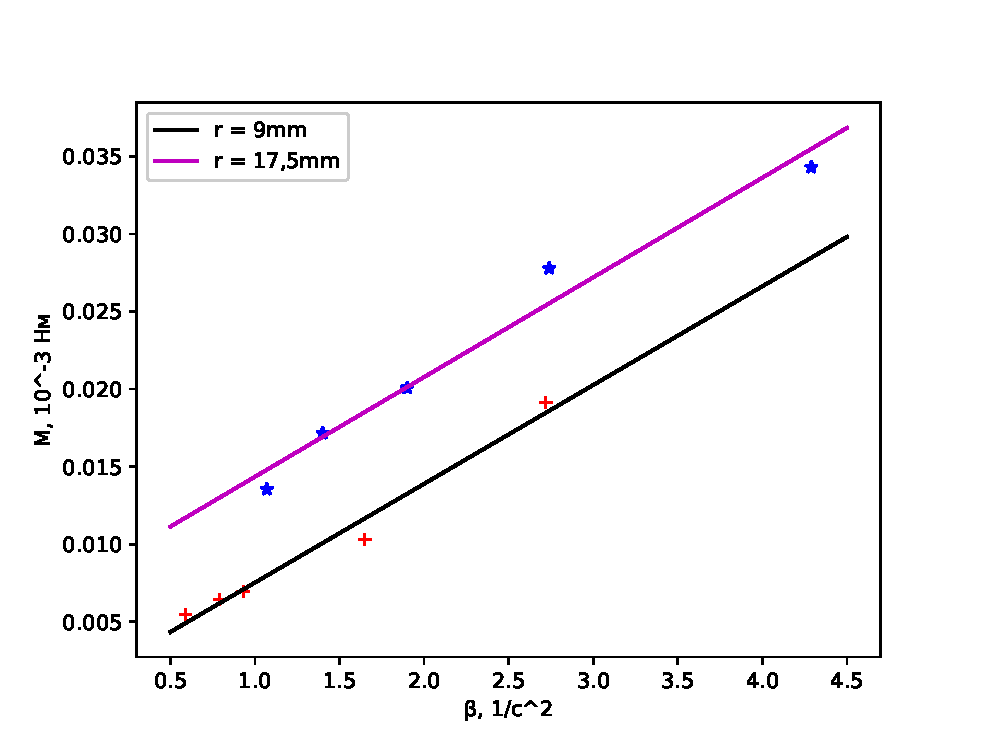
\includegraphics[scale = 0.7]{Plot.eps}

По МНК вычислим значения момента инерции:
\begin{align*}
I_1 = 6,36 \cdot 10^{-3} \pm 0,99 \cdot 10^{-3} \text{ кг$\cdot$м$^2$} \\
I_2 = 6,64 \cdot 10^{-3} \pm 1,27 \cdot 10^{-3} \text{ кг$\cdot$м$^2$}
\end{align*}

Оттуда же узнаем $M_T$:
\begin{align*}
M_T = M(0) \approx 5 \cdot 10^{-3} \text{ Нм}
\end{align*}

\subsection{Опыт №2. $R = 212,5$мм}

Запишем данные, полученные из экспериментов.
Рассчитаем для каждого эксперимента угловое ускорение $\beta$ и вращающий момент $M_H$:
\begin{align*}
\beta &= \frac{2h}{rt^2} \\
M_H &= mgr
\end{align*}

\begin{center}
\begin{tabular}{|c|p{4cm}|c|c|c|}
\hline
Диаметр шкива & Масса платформы с перегрузком & Время падения & $\beta$  & $M_0$       \\ \hline
мм            & г                             & с             & c$^{-2}$ & $10^{-3}$Нм \\ \hline
              & 79                            & 20            & 0,38     & 6,97        \\ \cline{2-5} 
              & 123                           & 18            & 0,46     & 9,64        \\ \cline{2-5} 
18            & 162                           & 15            & 0,60     & 12,70        \\ \cline{2-5} 
              & 217                           & 13            & 0,89     & 19,14       \\ \cline{2-5} 
              & 300                           & 11            & 1,24     & 23,52       \\ \hline \hline
              & 79                            & 13            & 0,41     & 13,55       \\ \cline{2-5} 
              & 100                           & 11            & 0,56     & 17,15       \\ \cline{2-5} 
35            & 124                           & 10            & 0,69     & 21,27       \\ \cline{2-5} 
              & 156                           & 8             & 1,07     & 26,75       \\ \cline{2-5} 
              & 200                           & 7             & 1,40     & 34,30       \\ \hline
\end{tabular}
\end{center}

Построим график зависимости $M$ от $\beta$

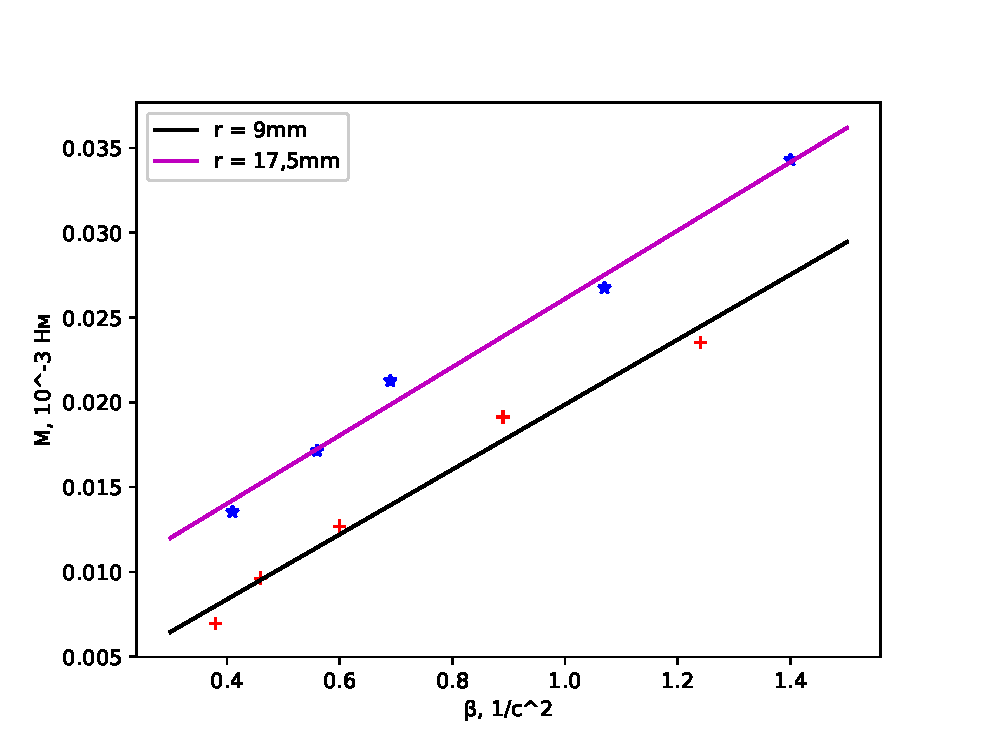
\includegraphics[scale = 0.7]{Plot2.eps}

По МНК вычислим значения момента инерции:
\begin{align*}
I_1 = 19,15 \cdot 10^{-3} \pm 1,6 \cdot 10^{-3} \text{ кг$\cdot$м$^2$} \\
I_2 = 20,14 \cdot 10^{-3} \pm 3,7 \cdot 10^{-3} \text{ кг$\cdot$м$^2$}
\end{align*}

Оттуда же узнаем $M_T$:
\begin{align*}
M_T = M(0) \approx 5 \cdot 10^{-3} \text{ Нм}
\end{align*}

\section{Вывод}

Из проведённых опытов видно, что зависимость углового ускорения от момента приложенных сил с достаточной точностью (8\%) аппроксимируется линейной функцией. Из чего можно сделать вывод, что формула $M = I\beta$ справедлива.

\end{document}